\documentclass[11pt]{beamer}
\usepackage[T1]{fontenc}
\usepackage[utf8]{inputenc}
\usepackage{lmodern}
\usepackage{tikz}
\usepackage{graphicx}
\usetheme{Madrid}
\usepackage[normalem]{ulem}
\usepackage[absolute,overlay]{textpos}
\usepackage{listings}
\usepackage{courier} 

\setbeamertemplate{navigation symbols}{}
%\setbeamertemplate{footline}[frame number]
\title[Main Title]{Main Title: very very extremely long title}
\subtitle{subtitle}
\author[k4iyer, ssasy, j3tracey]{K. Iyer \and S. Sasy \and J. Tracey}
\institute[]{Cheriton School of Computer Science}
\date{}


\newcommand*\circled[1]{\tikz[baseline=(char.base)]{
            \node[shape=circle,draw,inner sep=2pt] (char) {#1};}}

\begin{document}

\begin{frame}
  \titlepage
\end{frame}

\begin{frame}{Presentation Outline}
 	\begin{itemize}
          \vfill
        \item Types of Capabilities
          \vfill
        \item Capabilities in OSs
          \vfill
        \item Capabilities in Userspace
          \vfill
        \item Our Implementation
          \vfill
        \end{itemize}
\end{frame}

\begin{frame}{Types of Capabilities}
\begin{enumerate}
          \vfill
    \item{tagged with bits}
          \vfill
    \item{tagged with type system}
          \vfill
    \item{segregated}
          \vfill
    \item{password/sparse}
          \vfill
\end{enumerate}
\end{frame}

\begin{frame}{Types of Capabilities: The Roles}
  \begin{figure}[!h]
    \centering
    \begin{tikzpicture}
      \node (auth)[label=authority] at (0,0) {\includegraphics[scale=.025]{gavel.jpg}};
      \node (client)[label=client] at (-4,-4) {\includegraphics[scale=.15]{client.jpg}};
      \node (obj)[label=object] at (4,-4) {\includegraphics[scale=.075]{resource.jpg}};
    \end{tikzpicture}
  \end{figure}
\end{frame}

\begin{frame}{Types of Capabilities: Tagged with Bits}
  \begin{figure}[!h]
    \centering
    \begin{tikzpicture}
      \node (auth)[label=authority] at (0,0) {\includegraphics[scale=.025]{gavel.jpg}};
      \node (client)[label=client] at (-4,-4) {\includegraphics[scale=.15]{client.jpg}};
      \node (obj)[label=object] at (4,-4) {\includegraphics[scale=.075]{resource.jpg}};

      \draw[transform canvas={yshift=1.0ex}, draw=purple, very thick, <-] (auth) -- (client) node[above, left, midway] {?};
      \draw[transform canvas={yshift=-1.0ex}, draw=purple, very thick, ->] (auth) -- (client) node[below, right, midway] {\circled{T}};
      \draw[draw=purple, very thick, ->] (client) -- (obj) node[above, midway] {\circled{T}};
    \end{tikzpicture}
  \end{figure}
\end{frame}

\begin{frame}{Types of Capabilities: Tagged with Type System}
  \begin{figure}[!h]
    \centering
    \begin{tikzpicture}
      \node (auth)[label=authority] at (0,0) {\includegraphics[scale=.025]{gavel.jpg}};
      \node (client)[label=client] at (-4,-4) {\includegraphics[scale=.15]{client.jpg}};
      \node (obj)[label=object] at (4,-4) {\includegraphics[scale=.075]{resource.jpg}};

      \draw[transform canvas={yshift=1.0ex}, draw=purple, very thick, <-] (auth) -- (client) node[above, left, midway] {?};
      \draw[transform canvas={yshift=-1.0ex}, draw=purple, very thick, ->] (auth) -- (client) node[below, right, midway] {*};
      \draw[draw=purple, very thick, ->] (auth) -- (obj) node[above, right, midway] {\circled{C}};
      \draw[draw=purple, very thick, ->] (client) -- (obj) node[above, midway] {*};
    \end{tikzpicture}
  \end{figure}
\end{frame}


\begin{frame}{Types of Capabilities: Segregated}
  \begin{figure}[!h]
    \centering
    \begin{tikzpicture}
      \node (auth)[label=authority] at (0,0) {\includegraphics[scale=.025]{gavel.jpg}};
      \node (client)[label=client] at (-4,-4) {\includegraphics[scale=.15]{client.jpg}};
      \node (obj)[label=object] at (4,-4) {\includegraphics[scale=.075]{resource.jpg}};
      \node (book) at (1.5,0) {\includegraphics[scale=0.05]{alice.jpg}};

      \draw[draw=purple, very thick, <-] (auth) -- (client) node[above, left, midway] {``Alice''};
      \draw[draw=purple, very thick, ->] (auth) -- (obj) node[above, right, midway] {``Alice''};
    \end{tikzpicture}
  \end{figure}
\end{frame}

\begin{frame}{Types of Capabilities: Segregated}
  \begin{figure}[!h]
    \centering
    \begin{tikzpicture}
      \node (auth)[label=authority] at (0,0) {\includegraphics[scale=.025]{gavel.jpg}};
      \node (client)[label=client] at (-4,-4) {\includegraphics[scale=.15]{client.jpg}};
      \node (obj)[label=object] at (4,-4) {\includegraphics[scale=.075]{resource.jpg}};

      \draw[draw=purple, very thick, <-] (auth) -- (client) node[above, left, midway] {``passw0rd''};
      \draw[draw=purple, very thick, ->] (auth) -- (obj) node[above, right, midway] {``Alice''};
    \end{tikzpicture}
  \end{figure}
\end{frame}

\begin{frame}{Capabilities in OSs}
  \vfill
  A more in-depth look at two of these OSs:
  	\begin{itemize}
          \vfill
	\item L4
	\item Barrelfish
          \vfill
	\end{itemize}
\end{frame}

\begin{frame}{Capabilities in OSs: L4}

  	\begin{itemize}
          \vfill
	\item family of microkernels
          \vfill
	\item some use or are built on capabilities
          \vfill
        \item e.g. OKL4, Fiasco.OC, seL4
          \vfill
	\end{itemize}
\end{frame}

\begin{frame}{Capabilities in OSs: seL4}
  \vfill
  We focus on seL4 as the most relevant.
  \begin{itemize}
    \vfill
  \item first formally verified general-purpose OS
    \vfill
  \item minimizes kernel objects
    \vfill
  \item all kernel services managed using capabilities
    \vfill
  \end{itemize}
\end{frame}

\begin{frame}{Capabilities in OSs: seL4}
  The available kernel objects are categorized into:
  \begin{itemize}
    \vfill
  \item capabilities (CNodes, CSpaces)
    \vfill
  \item object/memory management (untyped $\rightarrow$ retyped)
    \vfill
  \item virtual address space management (VSpace, platform-dependant)
    \begin{itemize}
    \item e.g. IA32: Page Directory $\rightarrow$ Page Tables $\rightarrow$ Frames
    \end{itemize}
    \vfill
  \item thread management (Thread Control Block, TCB)
    \vfill
  \item inter-process communication (IPC, endpoints)
    \vfill
  \item device I/O management (ports, inturrupts, DMA address space)
    \vfill
  \end{itemize}
\end{frame}

\begin{frame}{Barrelfish: Overview}
	\begin{itemize}

	\item suitable for scalable operating systems 
		\vfill
	\item multi-cores architecture
		\vfill
	\item heterogeneous architecture
		\vfill
	\item extensions of the seL4 model for distributed capability management between cores
	\end{itemize}
\end{frame}


\begin{frame}{Barrelfish: Capability Types}
\begin{itemize}
\item Main Memory
\vfill
\item Page Tables 
\vfill
\item Device Memory
\vfill
\item Page tables Mapping Memory 
\vfill
\item Kernel interface
\vfill
\item Others
\end{itemize}
\end{frame}


\begin{frame}{Barrelfish: Capability Operations Interaction}
\begin{figure}
		  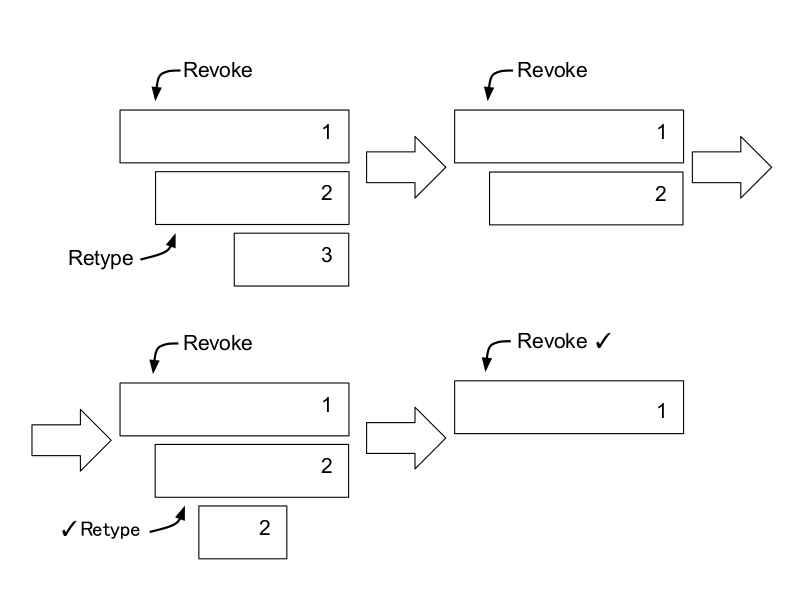
\includegraphics[scale=0.25]{img/BF_revoke_retype}
		  \caption{Revoke-Retype-Delete interactions}
		  
    \end{figure}   
\end{frame}

\begin{frame}{Capsicum: Overview}
	\begin{itemize}
	\item API for implementing capabilities on UNIX
	\vfill 
	\item extends (not replace) standard UNIX APIs by adding kernel-level primitives
	\vfill
	\item new OS primitives for implementing capabilities-
		\begin{itemize}
		    \item capabilities %- refined file descriptors with fine-grained rights
   		    \item capability mode% - process sandboxes that deny access to global namespaces
    		    \item process descriptors% - capability-centric process ID replacement
    		    \item anonymous shared memory objects% - an extension to the POSIX shared memory API to support anonymous swap objects associated with file descriptors (capabilities)
    		    \item rtld-elf-cap% - modified ELF run-time linker to construct sandboxed applications
    		    \item libcapsicum %- library to create and use capabilities and sandboxed components
    		    \item libuserangel %- library allowing sandboxed applications or components to interact with user angels, such as Power Boxes.
    		    \item chromium-capsicum %- a version of Google's Chromium web browser that uses capability mode and capabilities to provide effective sandboxing of high-risk web page rendering.

		\end{itemize}
	\end{itemize}
\end{frame}




\begin{frame}{Capsicum: Example}
	\begin{figure}
		  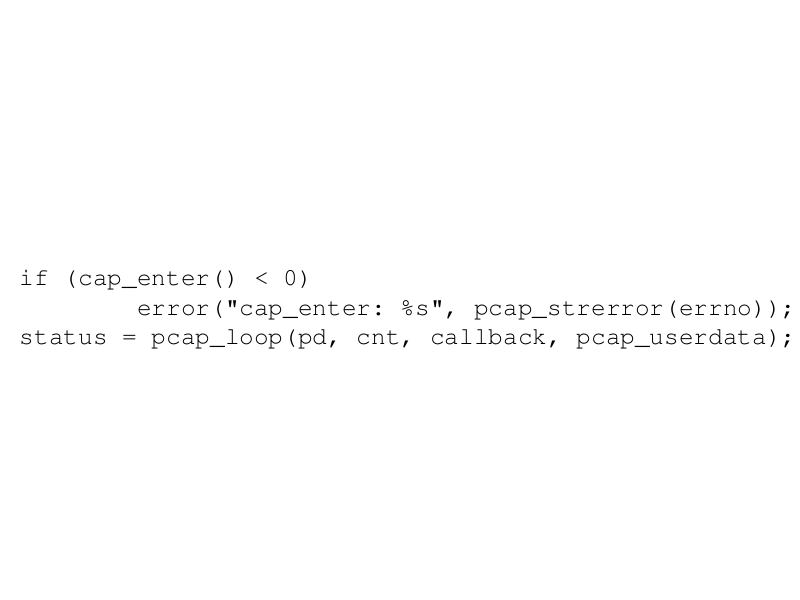
\includegraphics[scale=0.3]{img/tcpdump}
		  \caption{capsicum example}
		  
    \end{figure}  
\end{frame}


\begin{frame}{OrangeFS}
  \begin{columns}
    
  \begin{column}{.4\textwidth}
    \begin{itemize}
    \vfill
    \item Certificate based file system
    \vfill
    \item Model of capability with 
          tagged bits
    \vfill
    \item Data stored in clear
    \vfill
    \end{itemize}
  \end{column}
  
  \begin{column}{.6\textwidth}
    \begin{textblock*}{3cm}(6cm,3cm)
        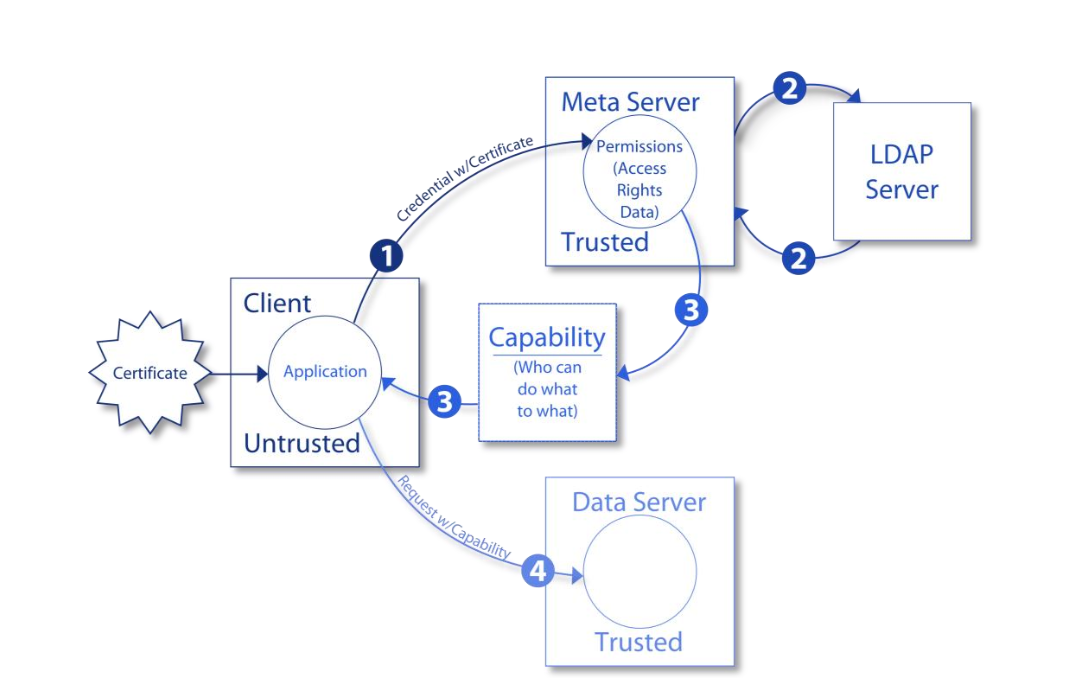
\includegraphics[width=6cm]{img/orange.png}
    \end{textblock*}
  \end{column}
  
  \end{columns}
\end{frame}

\begin{frame}{TahoeLAFS}
    \begin{itemize}
    \vfill
    \item Password based capability mode
    \vfill
    \item Mutable and Immutable files
    \vfill
    \item Directory Logic
    \vfill
    \end{itemize}
\end{frame}

\begin{frame}{TahoeLAFS (Immutable files)}
    \vfill
    \begin{itemize}
    \item Immutable Files
    \end{itemize}
    \vfill
    \begin{figure}
		  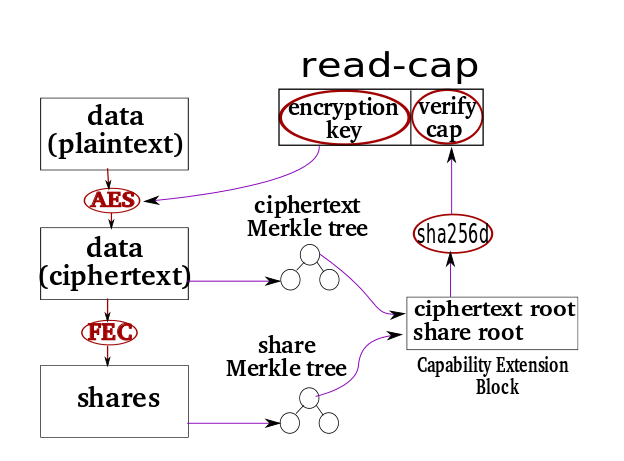
\includegraphics[scale=0.3]{img/immutable.png}
		  \caption{Handling Immutable Files in TahoeLAFS}
    \end{figure}
    \vfill
    % insert 1 diagram
\end{frame}

\begin{frame}{TahoeLAFS (Mutable files)}
    \vfill
    \begin{itemize}
    \item Mutable Files
    \end{itemize}
    \vfill
    \begin{figure}
		  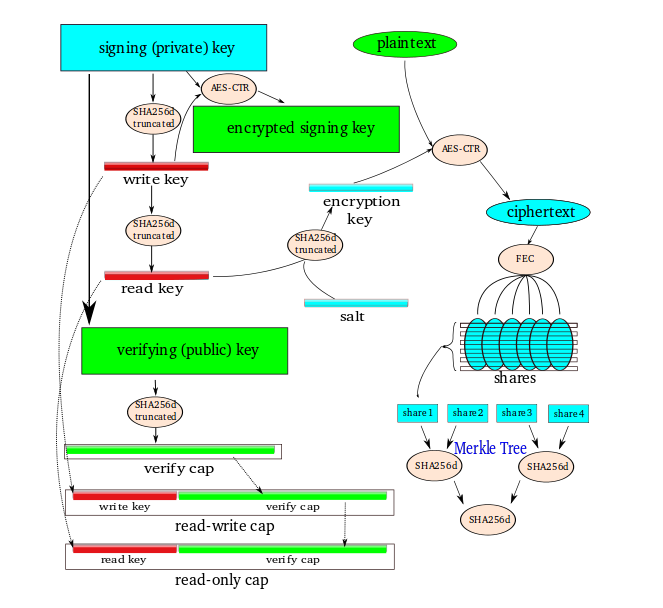
\includegraphics[scale=0.3]{img/mutable.png}
		  \caption{Handling Mutable file in TahoeLAFS}
    \end{figure}
    \vfill
\end{frame}

\begin{frame}{CapBAC}
    \begin{itemize}
    \vfill
    \item Designed for the Internet of Things
    \vfill
    \item JSON-file Tokens
    \vfill
    \end{itemize}
    \begin{textblock*}{2.5cm}(8cm,1.5cm)
        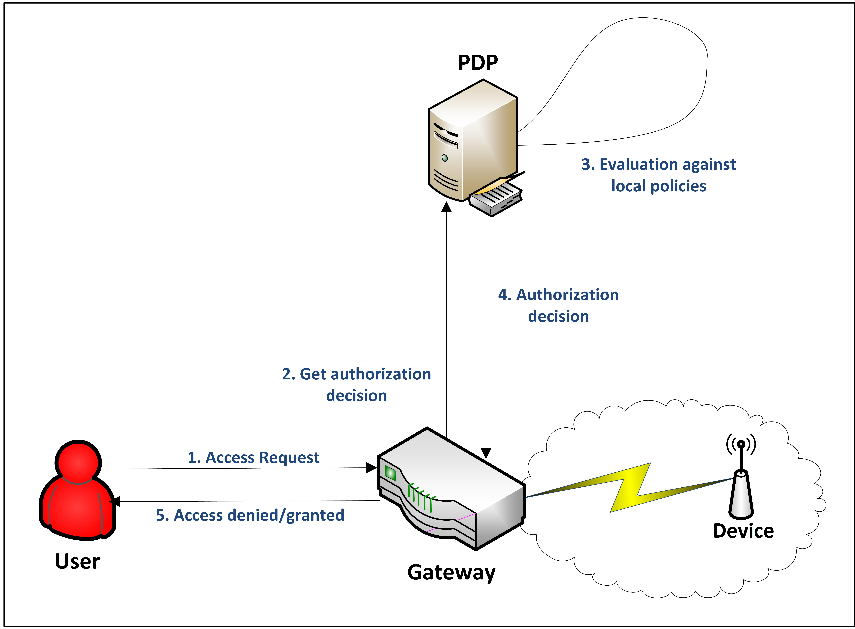
\includegraphics[width=4cm]{img/centralized.png}
    \end{textblock*}
    \begin{textblock*}{2.5cm}(8cm,5cm)
        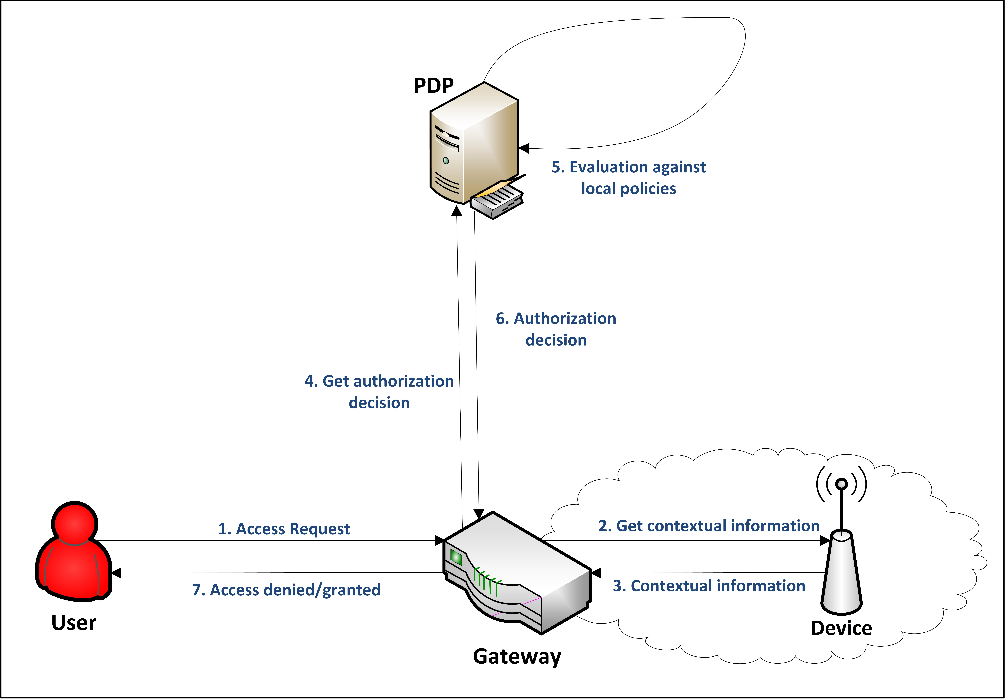
\includegraphics[width=4cm]{img/CAcentralized.png}
    \end{textblock*}
    \begin{textblock*}{2.5cm}(8cm,8cm)
        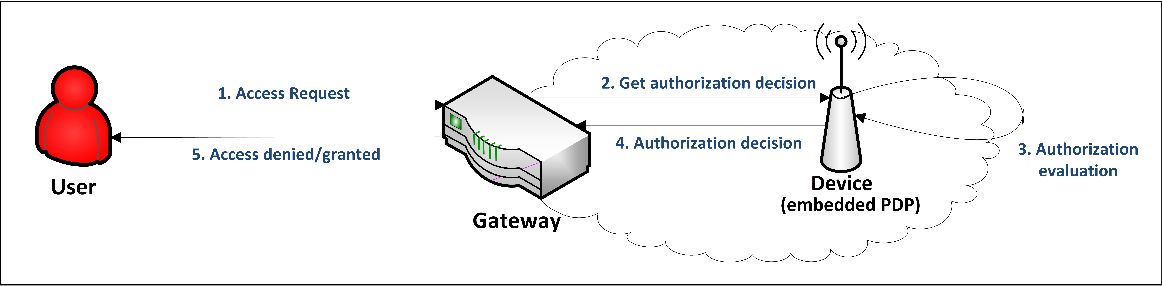
\includegraphics[width=4cm]{img/distributed.png}
    \end{textblock*}
    % insert 3 diagrams (centralized, CAcentralized, distributed)
\end{frame}


\begin{frame}{CapBAC}
    \vfill
    \begin{itemize}
    \item Implementation Model 
    \end{itemize}
        \vfill
    \begin{figure}
		  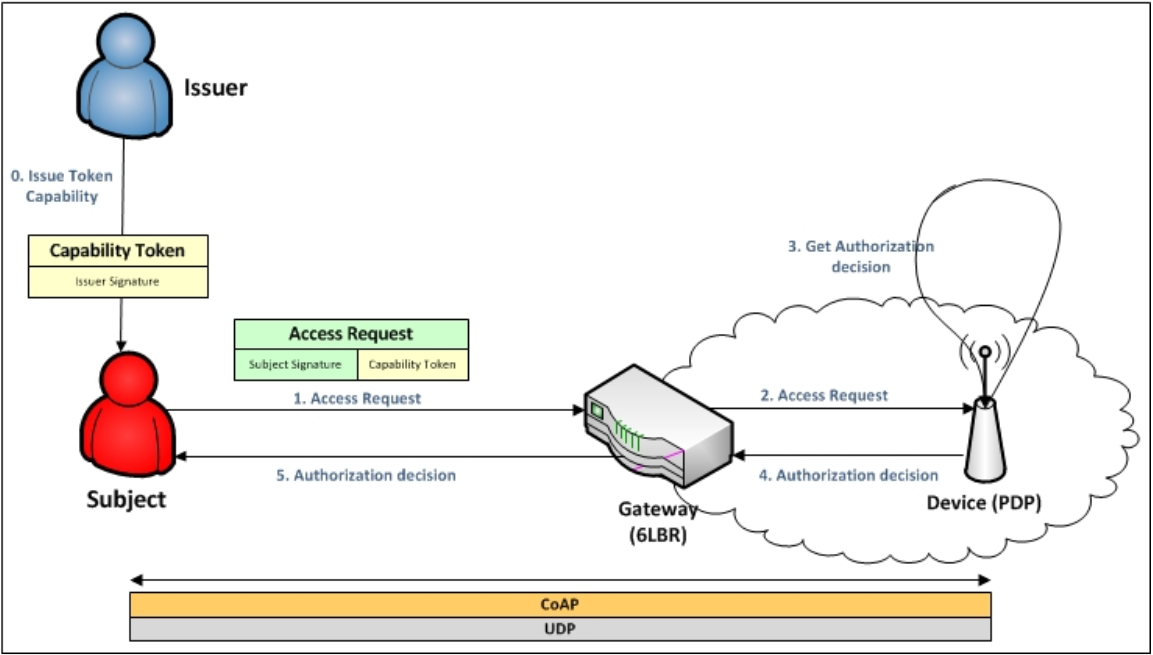
\includegraphics[scale=0.2]{img/capBac.png}
		  \caption{CapBAC Implementation Model}
    \end{figure}
    \vfill
    % insert 1 diagram capBAC
\end{frame}




\end{document}
